\documentclass[a4paper,11pt]{article}
\usepackage[utf8]{inputenc}
\usepackage[czech]{babel}
\usepackage[T1]{fontenc}
\usepackage{amsmath}
\usepackage{amsfonts}
\usepackage{amssymb}
\usepackage{graphicx}
\usepackage{mathtools}
\usepackage{fancyhdr}
\usepackage{epstopdf}
\usepackage{float}
\usepackage{gensymb}
\usepackage[final]{pdfpages}
\usepackage{a4wide}
\renewcommand{\arraystretch}{1.5}
%\renewcommand{\baselinestretch}{1.25}

\title{Automatické řízení \\
	Semestrální práce}
\usepackage[top=25mm, left=35mm, right=25mm, bottom=25mm]{geometry}
\author{Miroslav Bulka, Jan Cibulka}
\date{81.121.1025}	
\setlength{\parskip}{10pt}
\begin{document}
\maketitle

\begin{figure}[h]
	\centering
	
\includegraphics[width=9cm]{obrazky/fav.png}
\end{figure}
\clearpage
\newpage


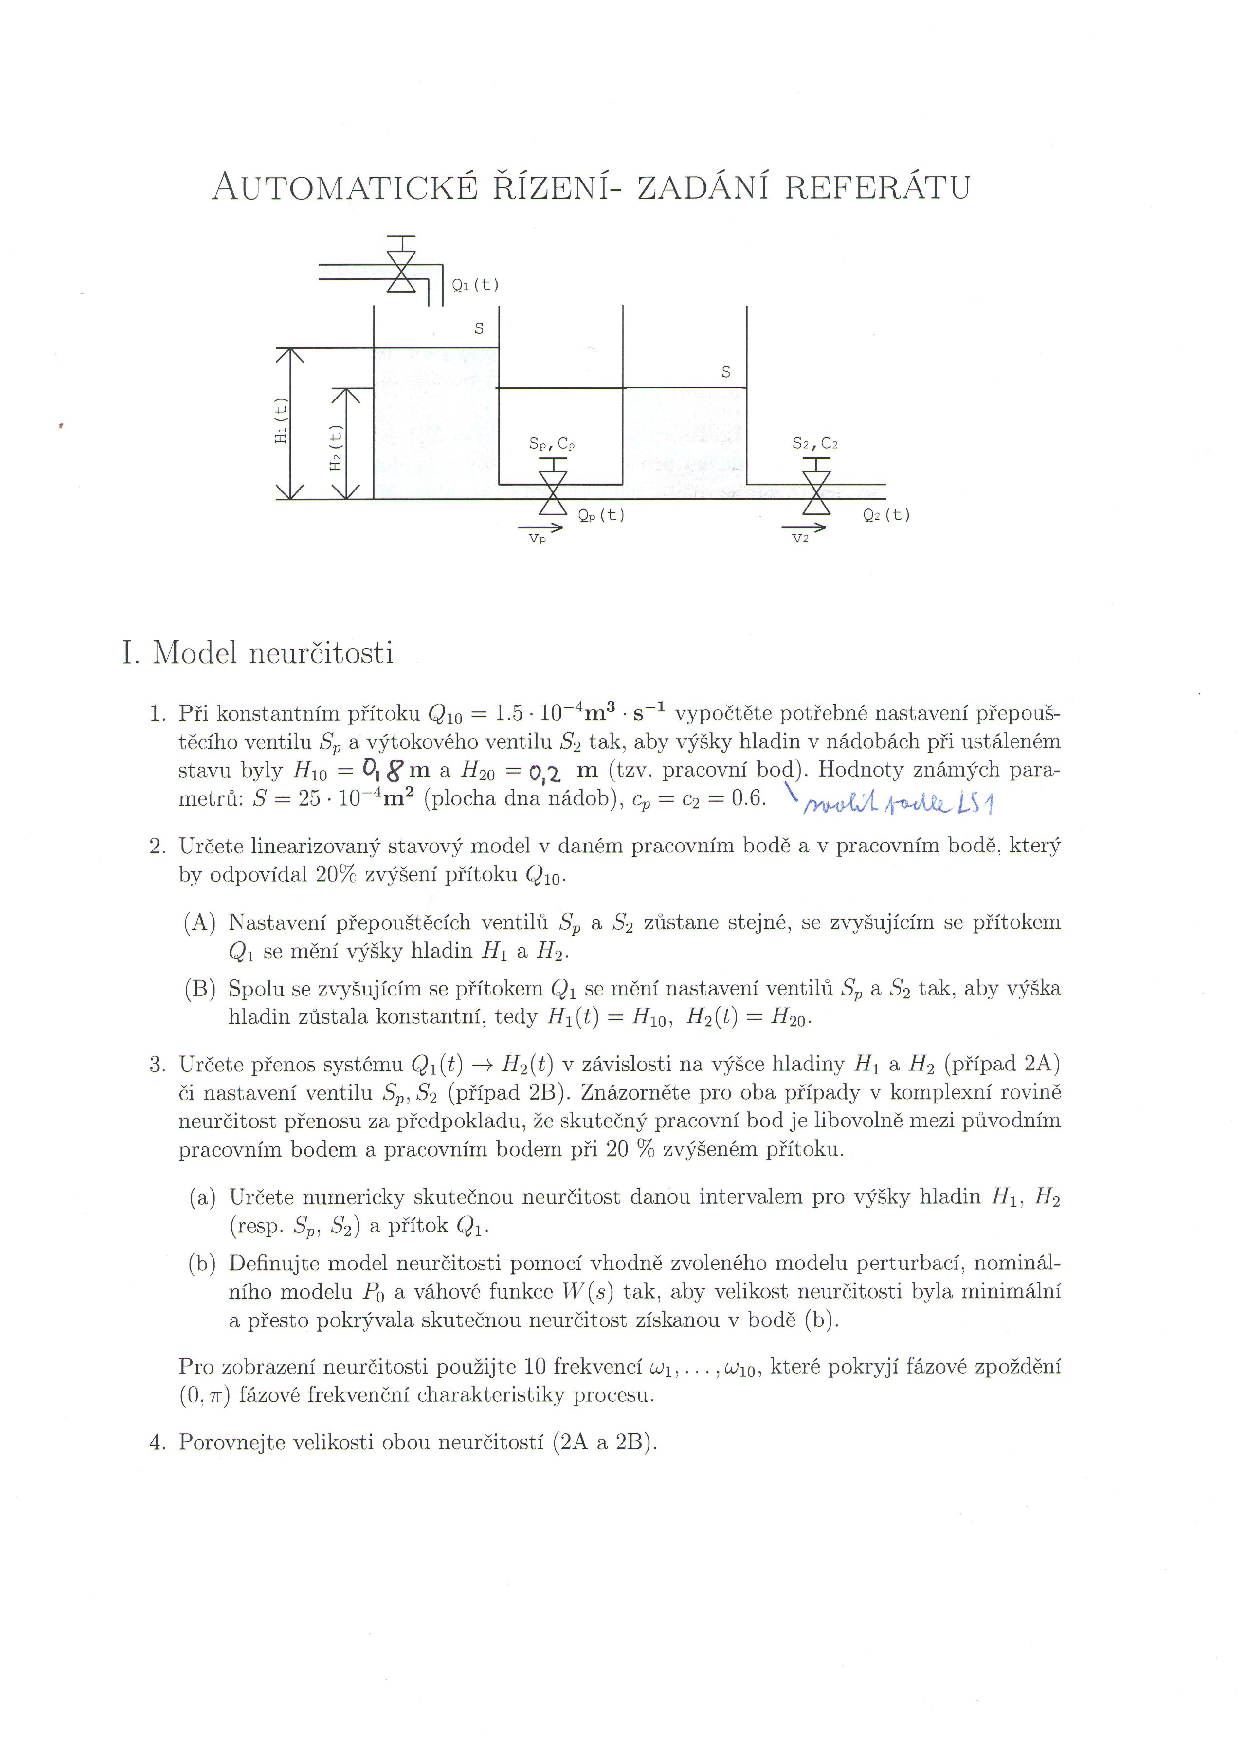
\includepdf{obrazky/Zadani1.pdf}
\newpage
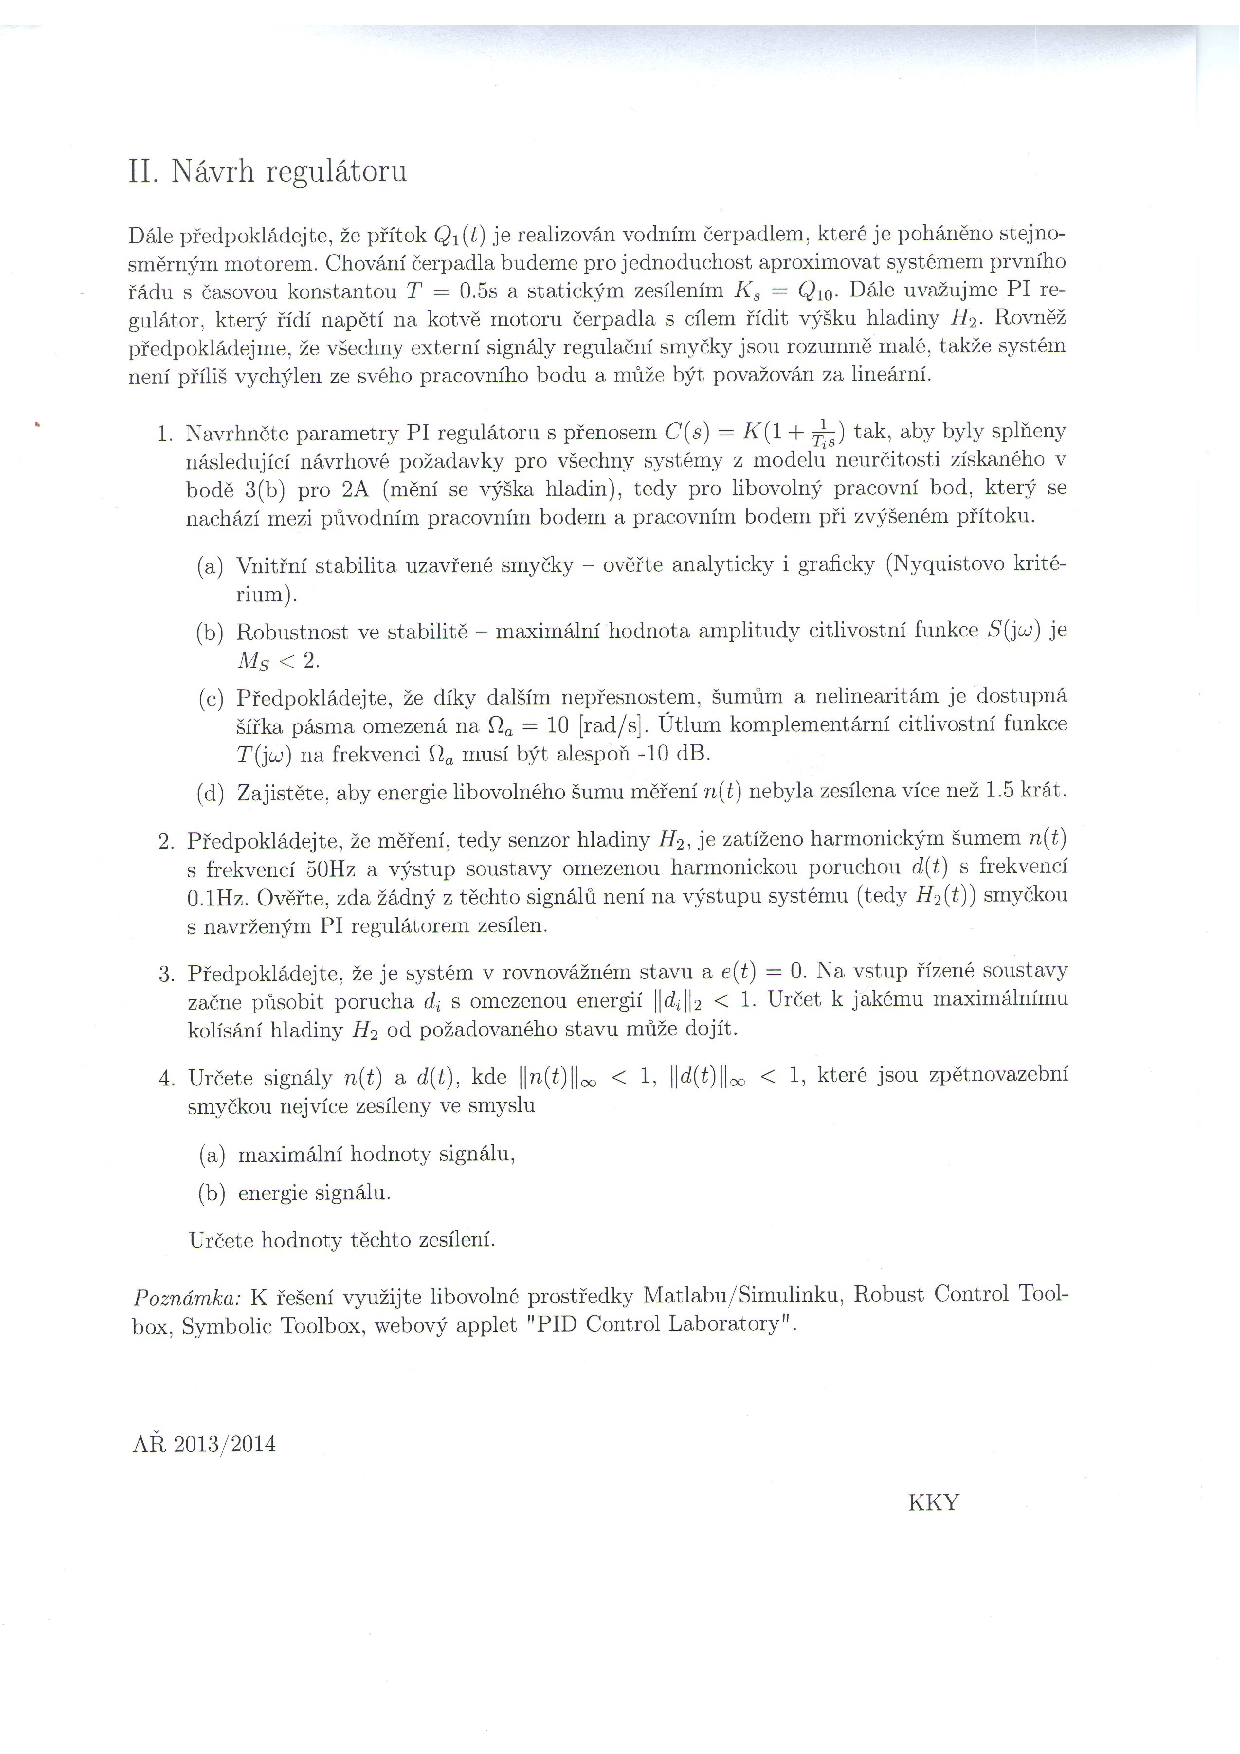
\includepdf{obrazky/Zadani2.pdf}
\newpage

\tableofcontents
\newpage
\section{Řešení - Model neurčitosti}
\subsection{První úkol - výpočet nastavení ventilů}
Máme konstantní přítok $Q_{1}=Q_{10}=1.5\cdot 10^{-4}m^{3}s^{-1}$, přičemž víme, že:
\begin{equation}
\left [\begin{array}{cc}
\frac{dV_{1}}{dt}\\
\frac{dV_{2}}{dt}
\end{array}\right ] = 
\left [\begin{array}{cc}
Q_{1}-Q_{p}\\
Q_{p}-Q_{2}\end{array}\right ] = 
\left [\begin{array}{cc}
Q_{1}-c_{p}S_{p}v_{p}\\
c_{p}S_{p}v_{p}-c_{2}S_{2}v_{2}\end{array}\right ].
\end{equation}
Z Bernoulliho zákona pak odvodíme:
\begin{equation}
\left [\begin{array}{cc}
v_{p} \\
v_{2}
\end{array}\right ] = 
\left [\begin{array}{cc}
\sqrt{2g\cdot (H_{1}-H_{2})}\\
\sqrt{2g\cdot (H_{2})}\end{array}\right ].
\end{equation}
Daný systém popisují diferenciální rovnice:
\begin{equation}
\left [\begin{array}{cc}
\frac{dH_{1}}{dt} \\
\frac{dH_{2}}{dt}
\end{array}\right ] = 
\left [\begin{array}{cc}
\frac{1}{S}\cdot Q_{1}-\frac{S_{p}C_{p}}{S}\cdot \sqrt{2g\cdot (H_{1}-H_{2})}\\
\frac{S_{p}C_{p}}{S}\cdot \sqrt{2g\cdot \left ( H_{1}-H_{2} \right )}-\frac{S_{2}C_{2}}{S}\cdot \sqrt{2g\cdot H_{2}}\end{array}\right ].
\end{equation}
Zavedením 
$ x_{1}(t)=H_{1}(t);\;$ 
$x_{2}(t)=H_{2}(t);\;$ 
$u(t)=Q_{1}(t)\; $
získáme
\begin{equation}\label{eq:Stavove_x} 
\left [\begin{array}{cc}
\frac{dx_{1}}{dt} \\
\frac{dx_{2}}{dt}
\end{array}\right ] = 
\left [\begin{array}{cc}
\frac{1}{S}\cdot u-\frac{S_{p}C_{p}}{S}\cdot \sqrt{2g\cdot (x_{1}- x_{2})}\\
\frac{S_{p}C_{p}}{S}\cdot \sqrt{2g\cdot \left ( x_{1}-x_{2} \right )}-\frac{S_{2}C_{2}}{S}\cdot \sqrt{2g\cdot x_{2}}\end{array}\right ].
\end{equation}
Za předpokladu neměnících se hladin $H_{1}$ a $ H_{2} $ budou obě derivace nulové. Položíme je tedy nulou a díky tomu získáme požadované nastavení přepouštěcího ventilu $S_{p}$ a výtokového ventilu $S_{2}$:
\begin{equation}\label{eq:vypocet_ventilu}
\left [\begin{array}{cc}
S_{p} \\
S_{2}
\end{array}\right ] = 
\left [\begin{array}{cc}
\frac{Q_{10}}{C_{p}\cdot \sqrt{2g\left ( H_{1}-H_{2} \right )}}\\
\frac{C_{p} S_{p}\sqrt{\left ( H_{1}-H_{2} \right )}}{C_{2} \sqrt{H_{2}}}\end{array}\right ],
\end{equation}
kde po dosazení získáme:
\begin{equation}\label{eq:nastaveni_ventilu_10}
\left [\begin{array}{cc}
S_{p} \\
S_{2}
\end{array}\right ] = 
\left [\begin{array}{cc}
7.2864\cdot 10^{-5}\\
1.2620\cdot 10^{-4}\end{array}\right ].
\end{equation}

\newpage 
\subsection{Druhý úkol - linearizace ve dvou pracovních bodech}\label{sec:2}
\subsubsection{Konstantní průtoky - mění se hladina}
\label{sec:2A}
Nejdříve si zavedeme značení:
\begin{equation}
\left [\begin{array}{cc}
y_{1}\left ( t \right ) \\
y_{2}\left ( t \right )
\end{array}\right ] = 
\left [\begin{array}{cc}
x_{1}\left ( t \right )\\
x_{2}\left ( t \right )\end{array}\right ]=
\left [\begin{array}{cc}
H_{1}\left ( t \right )\\
H_{2}\left ( t \right )\end{array}\right ].
\end{equation}
Chování těchto stavových proměnných je popsáno rovnicí \ref{eq:Stavove_x}. My chceme získat linearizovaný stavový model, a to ve tvaru:
\begin{equation}
\dot{x}\left ( t \right )=Ax\left( t \right )+Bu \left( t \right)\end{equation}
\begin{equation}
y\left ( t \right )=Cx\left( t \right ).
\end{equation}
Pro systém popsaný rovnicí \ref{eq:Stavove_x} budou parametry  linearizovaného stavového modelu, provedeme-li klasickou linearizaci, mít následující podobu:
\begin{equation}\label{eq:linearizace_zakladni_vztah}A = 
\left [\begin{array}{cc}
-\frac{C_{p}S_{p}\sqrt{2g}}{2\cdot S\sqrt{\left ( H_{1}-H_{2} \right )}} & \frac{C_{p}S_{p}\sqrt{2g}}{2\cdot S\sqrt{\left ( H_{1}-H_{2} \right )}} \\
\frac{C_{p}S_{p}\sqrt{2g}}{2\cdot S\sqrt{\left ( H_{1}-H_{2} \right )}} & -\frac{C_{p}S_{p}\sqrt{2g}}{2\cdot S\sqrt{\left ( H_{1}-H_{2} \right )}}-\frac{C_{2}S_{2}g}{S\sqrt{\left ( 2\cdot g\cdot H_{2} \right )}}
\end{array}\right ].
\end{equation}
\begin{equation}B = 
\left [\begin{array}{cc}
\frac{1}{S}\\
0
\end{array}\right ].
\end{equation}
Parametry modelu pro konstantní přítok $Q_{1}=Q_{10}=1.5\cdot 10^{-4}m^{3}s^{-1}$:
$$A =
\left [\begin{array}{cc}
-0.05  & 0.05 \\
0.05 & -0.2
\end{array}\right ];\;
B= 
\left [\begin{array}{cc}
400\\
0\end{array}\right ];\;
C=
\left [\begin{array}{cc}
1 & 0\\
0 & 1\end{array}\right ].
$$
Parametry modelu pro zvýšený přítok $Q_{20}=Q_{10}\cdot1.2=1.8\cdot 10^{-4}m^{3}s^{-1}$:
$$A =
\left [\begin{array}{cc}
-0.0417  & 0.0417 \\
0.0417 & -0.1667
\end{array}\right ];\;
B= 
\left [\begin{array}{cc}
400\\
0\end{array}\right ];\;
C=
\left [\begin{array}{cc}
1 & 0\\
0 & 1\end{array}\right ].
$$
\subsubsection{Konstantní hladina - mění se průtoky}\label{sec:2B}
V tomto případě budeme usilovat o to, aby se hladiny neměnily.
Bude tedy platit: 
\begin{equation}
\left [\begin{array}{cc}
H_{1}\left ( t \right ) \\
H_{2}\left ( t \right )
\end{array}\right ] = 
\left [\begin{array}{cc}
H_{10}\\
H_{20}\end{array}\right ].
\end{equation}
Naopak budeme měnit nastavení ventilů. Takovéto nastavení jsme pro konstantní přítok $ Q_{10} $ již spočetli, viz výsledek \ref{eq:nastaveni_ventilu_10}. Aby byla výška hladin konstantní i při přítoku $ 1.2 \cdot Q_{10} $, budeme muset nastavení ventilů přepočítat pomocí vztahu \ref{eq:vypocet_ventilu}, čímž získáme následující výsledné nastavení:
\begin{equation}\label{eq:nastaveni_ventilu_20}
\left [\begin{array}{cc}
S_{p} \\
S_{2}
\end{array}\right ] = 
\left [\begin{array}{cc}
8.7437\cdot 10^{-5}\\
1.5145\cdot 10^{-4}\end{array}\right ].
\end{equation}
K získání linearizovaného stavového modelu v tomto pracovním bodě využijeme zavedeného vztahu \ref{eq:linearizace_zakladni_vztah}. Jeho parametry budou vypadat následovně:
$$A =
\left [\begin{array}{cc}
-0.06  & 0.06 \\
0.06 & -0.24
\end{array}\right ];\;
B= 
\left [\begin{array}{cc}
400\\
0\end{array}\right ];\;
C=
\left [\begin{array}{cc}
1 & 0\\
0 & 1\end{array}\right ].
$$

\newpage 
\subsection{Třetí úkol - určení přenosu systému}\label{sec:3}
Nyní nás zajímá přenos systému $ Q_{1}\left ( t \right )\rightarrow H_{2}\left ( t \right ) $. Je tedy zřejmé, že měříme pouze veličinu $ H_{2}\left ( t \right ) $. Matici $ C $ stavového popisu
\begin{equation}
\dot{x}\left ( t \right )=Ax\left( t \right )+Bu \left( t \right)\end{equation}
\begin{equation}
y\left ( t \right )=Cx\left( t \right )
\end{equation}
budeme nyní uvažovat jako: $$C=\left [\begin{array}{cc}0 & 1\end{array}\right ].
$$
Přenos systému poté určíme ze stavové rovnice linearizovaného modelu pomocí známého vztahu:
\begin{equation}\label{eq:stav_popis} 
P\left ( s \right )=C\cdot \left ( sI-A \right )^{-1}\cdot B.
\end{equation}
V kapitolách \ref{sec:2A} a \ref{sec:2B} jsme získali tři různé stavové reprezentace pro různé situace, jako jsou různá nastavení ventilů a přítoků. Nejdříve spočteme přenosy pro systém popsaný v kapitole \ref{sec:2A}, tedy pro přítok $ Q_{10} $ ($ P_{1}\left ( s \right )  $) a pro jeho zvýšenou variantu ($ P_{2}\left ( s \right )  $):
\begin{equation}\label{eq:P-A1} 
P_{1}\left ( s \right ) =\frac{20}{s^{2} + 0.25 s + 0.0075}
\end{equation}
\begin{equation}\label{eq:P-A2} 
P_{2}\left ( s \right ) =\frac{16.67}{s^{2} + 0.2083  s + 0.005208},
\end{equation}
jejichž znázornění v komplexní rovině si můžeme prohlédnout na obrázku \ref{fig:nyquist-A}.
\begin{figure}[htbp]
	\begin{center}
	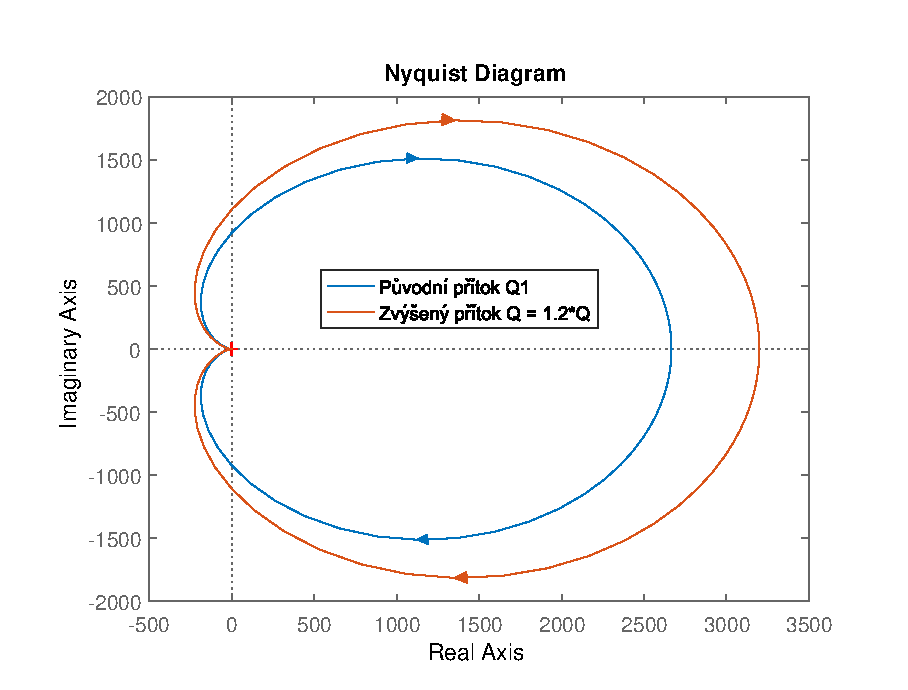
\includegraphics[scale = 1.0]{obrazky/nyquistA.eps}
	\caption{Nyquistova frekvenční charakteristika pro dané přenosy.}
	\label{fig:nyquist-A}
	\end{center}
\end{figure}

\newpage 
Pro získání přenosů pro systém popsaný v kapitole \ref{sec:2B} budeme postupovat stejně a získáme znovu dva přenosy pro pro přítok $ Q_{10} $ ($ P_{1}\left ( s \right )  $) a pro jeho zvýšenou variantu ($ P_{2}\left ( s \right )  $):
\begin{equation}\label{eq:P-B1} 
P_{1}\left ( s \right ) =\frac{20}{s^{2} + 0.25 s + 0.0075}
\end{equation}
\begin{equation}\label{eq:P-B2} 
P_{2}\left ( s \right ) =\frac{24}{s^{2} + 0.3  s + 0.0108},
\end{equation}
jejichž znázornění v komplexní rovině si můžeme prohlédnout na obrázku \ref{fig:nyquist-B}.
\begin{figure}[htbp]
	\begin{center}
	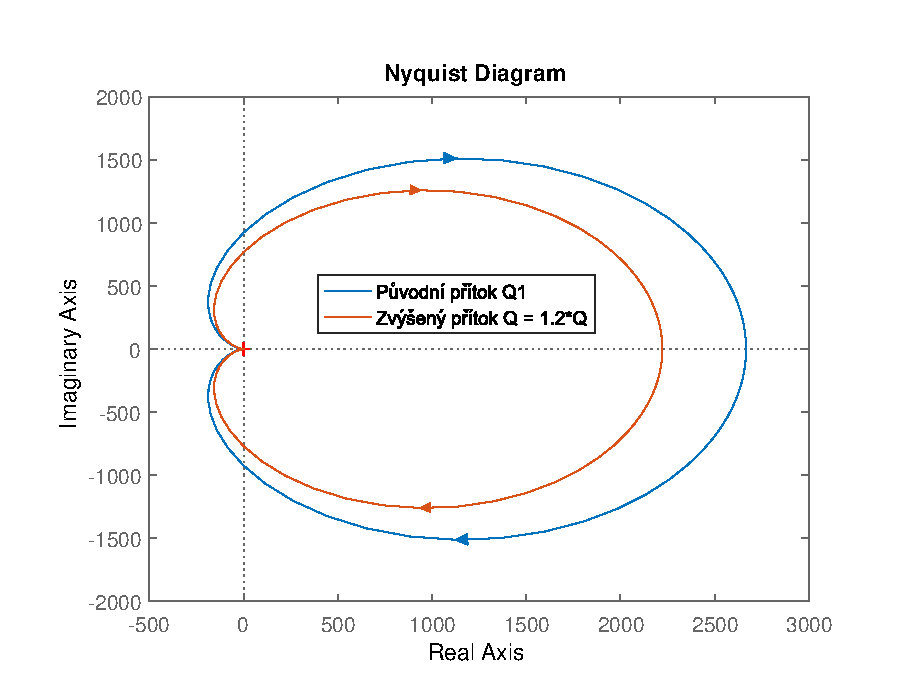
\includegraphics[scale = 1.0]{obrazky/nyquistB.eps}
	\caption{Nyquistova frekvenční charakteristika pro dané přenosy.}
	\label{fig:nyquist-B}
	\end{center}
\end{figure}

\newpage 
\subsubsection{Určení numerické neurčitosti}
Nyní budeme uvažovat, že máme množinový model, ve kterém jsou všechny přenosy $ P $, které vznikly z nominálního přenosu $ P_{0} $ aditivní perturbací:
\begin{equation}\label{eq:Aditivni_neurcitost-zakladni_vztah} 
P = P_{0}+W_{a}\Delta,
\end{equation}
kde $ \left\| \Delta   \right \|_{_{\infty }}< 1 $ a $ W_{a}\left ( s \right ) $ je pevně daná přenosová funkce. Tu můžeme vyjádřit následujícím způsobem:
\begin{equation}\label{eq:Vahova_fce_aditvni} 
W_{a}\left ( s \right ) = P_{0}\left ( s \right )-P\left ( s \right ),
\end{equation}
kde za $ P\left ( s \right ) $ budeme dosazovat přenosy spočtené výše, tedy výsledky \ref{eq:P-A1}, \ref{eq:P-A2}, \ref{eq:P-B1} a \ref{eq:P-B2}. Nejprve se tedy zabývejme přenosy týkající se varianty A, tedy přenosy $ P_{1}\left ( s \right ) $ pro $ Q_{10} $ (viz \ref{eq:P-A1}) a $ P_{1}\left ( s \right ) $ pro $ 1.2\cdot Q_{10} $ (viz \ref{eq:P-A2}) , které jsme spočetli výše. Dále předpokládáme, že pracovní bod se nachází libovolně mezi těmito dvěma pracovními body, lišící se v přítoku $ Q $. Je zřejmé, že nominální model bude vhodné určit pro pracovní bod ležící zhruba uprostřed tohoto intervalu, tedy pro konstantní přítok $ 1.1\cdot Q_{10} $. Při jeho určení budeme postupovat stejně jako během určování $ P_{1}\left ( s \right ) $ a $ P_{2}\left ( s \right ) $. Nominální přenos tedy bude mít tvar:
\begin{equation}\label{eq:P-A0} 
P_{0}\left ( s \right ) =\frac{18.18}{s^{2} + 0.2273 s + 0.006198}.
\end{equation}
Váhovou funkci pro námi zvolenou aditivní neurčitost spočteme ze vztahu \ref{eq:Vahova_fce_aditvni}:   
\begin{equation}\label{eq:Wa-A}
Wa = \frac{1.818 s^{2} + 8.882\cdot 10^{-16}s - 0.0124}{s^{4} + 0.4773 s^{3} + 0.07052 s^{2} + 0.003254 s + 4.649\cdot 10^{-5}}.
\end{equation} 
Zajímavé bude zejména grafické znázornění neurčitosti. To provedeme pro různé kombinace přenosových funkcí, které odpovídají systému za předpokladu různých velikostí konstantních přítoků, přičemž zavedeme omezení: 
\begin{equation}
\label{eq:Q_omezeni} 
Q_{10} \leq Q_{1} \leq 1.2\cdot Q_{10}, 
\end{equation}
z nichž jednomu bude odpovídat námi zvolení nominální model $ P_{0} $. Zobrazení k komplexní rovině je ke shlédnutí na obrázku \ref{fig:neurcitost-A}.
\begin{figure}[htbp]
	\begin{center}
	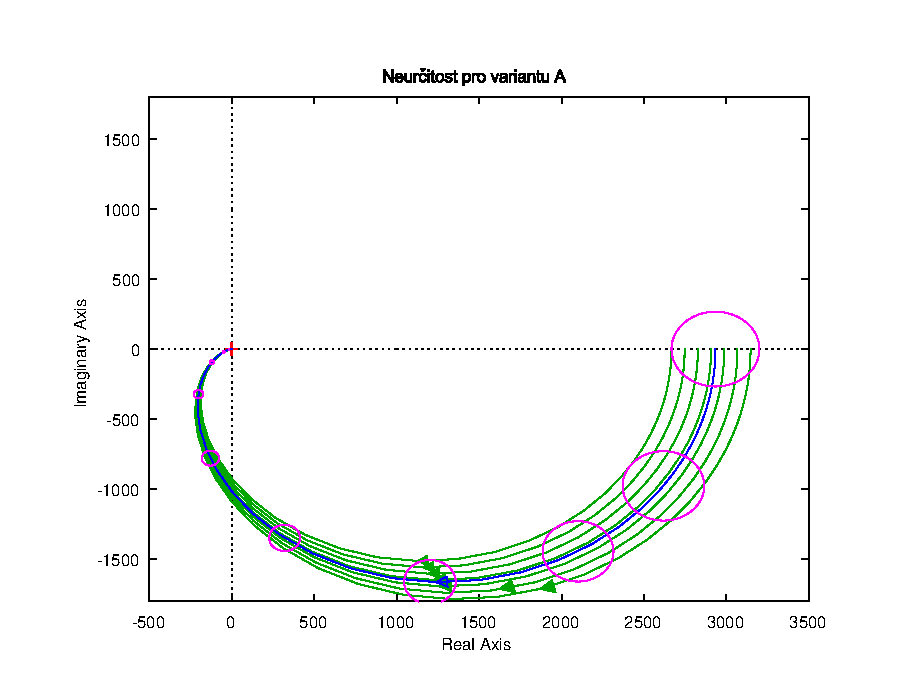
\includegraphics[scale = 1.0]{obrazky/neurcitostA.eps}
	%\caption{}
	\label{fig:neurcitost-A}
	\end{center}
\end{figure}

S přenosy $ P_{1}\left ( s \right ) $ a $ P_{2}\left ( s \right ) $ týkajícími se varianty B (viz tvary přenosů \ref{eq:P-B1} a \ref{eq:P-B2}) budeme pracovat stejně. V tomto případě bude mít nominální přenos tvar:
\begin{equation}\label{eq:P-B0} 
P_{0}\left ( s \right ) =\frac{22}{s^{2} + 0.275 s + 0.009075},
\end{equation}
načež dále opět využijeme vztahu \ref{eq:Vahova_fce_aditvni} k určení váhové funkce:
\begin{equation}\label{eq:Wa-B}
Wa = \frac{-2s^{2} + 8.882\cdot 10^{-16}s - 0.0165}{s^{4} + 0.525 s^{3} + 0.08532 s^{2} + 0.004331 s + 6.806\cdot 10^{-5}}.
\end{equation}
Grafické znázornění provedeme rovněž stejně jako v předchozím bodě za respektování omezení \ref{eq:Q_omezeni}. Znázornění je možno vidět na obrázku \ref{fig:neurcitost-B}.
\begin{figure}[htbp]
	\begin{center}
	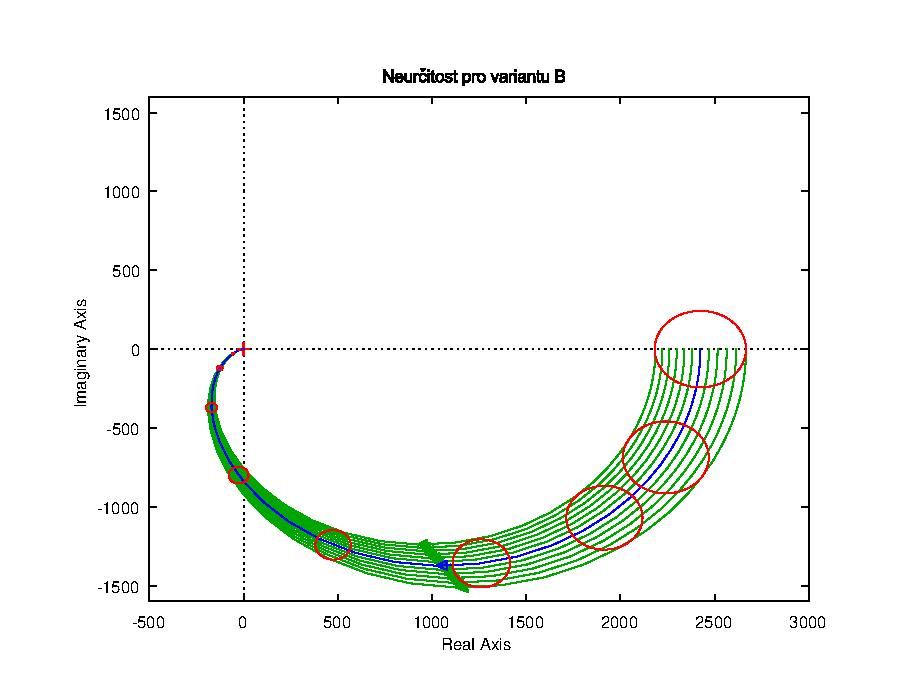
\includegraphics[scale = 1.0]{obrazky/neurcitostB.eps}
	%\caption{}
	\label{fig:neurcitost-B}
	\end{center}
\end{figure}

\newpage
Na obrázcích \ref{fig:neurcitost-A} a \ref{fig:neurcitost-B} si všimněme, že je zde vykresleno několik zelených křivek pro přenosové funkce za předpokladu různých, na intervalu \ref{eq:Q_omezeni} vhodně rozmístěných, konstantních přítoků. Modrá křivka představuje náš nominální model $ P_{0} $. V případě aditivní perturbace se velikost neurčitosti rovná $ \left | W_{a} \right | $, která určuje poloměr kružnic, které mají střed na křivce značící nominální přenos. na orázcích jich vidíme hned několik, a to pro vhodně zvolené frekvence $ \omega $.

\subsection{Čtvrtý úkol - Porovnání velikostí neurčitostí}
Porovnání neurčitostí pro oba případy provedeme vykreslením příslušných Bodeho frekvenčních charakteristik, kde pozorujeme nepatrné rozdíly, viz obrázek \ref{fig:porovnani_neurcitosti}.
\begin{figure}[htbp]
	\begin{center}
	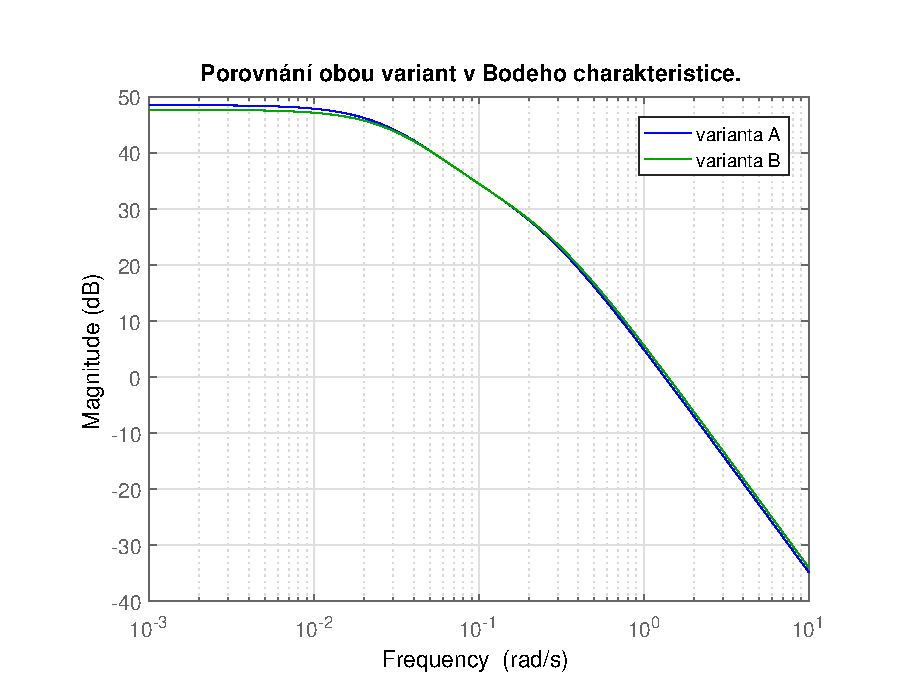
\includegraphics[scale = 1.0]{obrazky/porovnaniNeurcitosti.eps}
	%\caption{}
	\label{fig:porovnani_neurcitosti}
	\end{center}
\end{figure}


\newpage
\section{Řešení - Návrh regulátoru}
\subsection{První úkol}
Parametry PI regulatoru. Nejsem si jistej jestli tady jde o subukoly nebo jenom podminky pro jeden ukol.
\subsubsection{Vnitřní stabilita uzavřené smyčky (Nquistovo kritérium)}
\subsubsection{Robustnost ve stabilitě}
\subsubsection{Podmínka útlumu komplementrání citlivostní funkce}
\subsubsection{Energie šumu omezená.}
\subsection{Druhý úkol}
Harmonické poruchy.
\subsection{Třetí úkol}
Maximální kolísání hladiny.
\subsection{Čtvrtý úkol}
Určení hodnoty nějakých signálů.


\end{document}      
